%%%%%%%%%%%%%%%%%%%%%%%%%%%%%%%%%%%%%%%%%%%%%%%%%%%%%%%%%%%%%%%%%%%%%%%%%%%%%%%%%%%
% 			Facultad de Ciencias, UAEM.							Agosto de 2013
% 
%	Alumno: 				Emanuel García Perez
%	Asginatura:				Computación y Sociedad
%	Proyecto:				Exposición
%	Tema:					"OpenNet Initiative"
%
%%%%%%%%%%%%%%%%%%%%%%%%%%%%%%%%%%%%%%%%%%%%%%%%%%%%%%%%%%%%%%%%%%%%%%%%%%%%%%%%%%%


\documentclass{beamer}

\usepackage[spanish,activeacute]{babel}
\usepackage[latin1]{inputenc}
\usepackage{beamerthemeshadow}
\usepackage{graphicx}

\title{\textbf{OpenNet Initiative}}
\author{Emanuel Garc\'ia P\'erez}
\date{\today}

\begin{document}

\frame[allowframebreaks]{\titlepage}
\section[Contenidos]{}
\frame{
\transdissolve[duration=0.2]
\tableofcontents
}


\section{La OpenNet Initiative}
\subsection{?`Qu\'e es OpenNet Initiative?}
\frame
{
\transdissolve[duration=0.2]
\frametitle{OpenNet Initiative}
La OpenNet Initiative es una asociaci\'on que esta integrada por tres instituciones colaborativas: el Citizen Lab of the Munk School of Global Affairs, Universidad de Toronto; el Berkman Center for Internet \& Society, Universidad de Harvard; y el SecDev Group, Ottawa.\\
El objetivo de esta asociaci\'on es investigar, analizar y exponer el filtrado de Internet as\'i como tambi\'en las practicas de vigilancia de una manera sostenible.
\begin{figure}
  \centering
    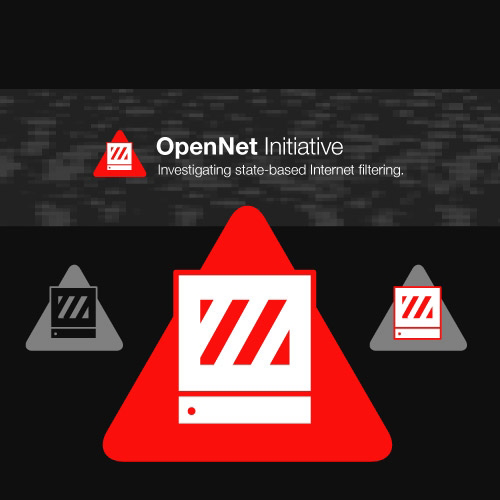
\includegraphics[width=0.3\textwidth]{oni.png}
  \label{fig:ejemplo}
\end{figure}
}

\frame
{
\transdissolve[duration=0.2]
\frametitle{El prop\'osito de la ONI}
Mediante el empleo de un enfoque multidiciplinario, la ONI se encarga de investigar, analizar y exponer las pr\'acticas de filtrado y vigilancia en Internet, de una manera cre\'ible y sustentable. Teniendo como intenci\'on descubrir los peligros y las consecuencias potenciales de estas pr\'acticas de censura y filtrado.
\begin{figure}
  \centering
    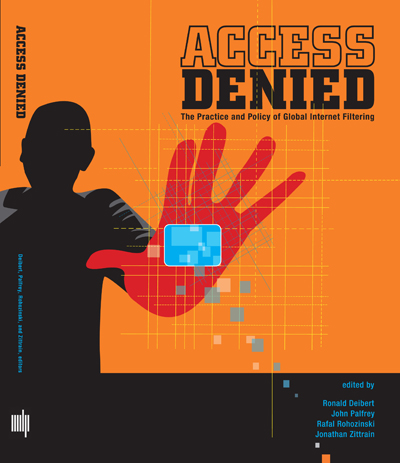
\includegraphics[width=0.35\textwidth]{img.jpg}
  \label{fig:ejemplo}
\end{figure}
}


\section{Filtrado en Internet}
\frame
{
\transdissolve[duration=0.2]
\frametitle{La censura de Internet}
La censura y restricciones de contenidos en Internet se lleva a cabo mediante diversas estrategias. El filtrado propiamente dicho, hace referencia a hacia aquellos criterios t\'ecnicos utilizados para controlar el acceso a la informaci\'on.
\begin{figure}
  \centering
    
\includegraphics[width=0.5\textwidth]{cens_web.jpg}
  \label{fig:ejemplo}
\end{figure}
}

\subsection{Enfoques de Filtrado}

\frame
{
\transdissolve[duration=0.2]
\frametitle{TECHNICAL BLOCKING}
Bloqueo de IP, manipulaci\'on de DNS y bloqueo de URL mediante proxy, son las t\'ecnicas que m\'as se utilizan para bloquear el acceso a determinadas p\'aginas web, ciertos dominios o direcciones IP. Tambi\'en podemos encontrar entre las principales t\'ecnicas empleadas el bloqueo por palabras clave y ataques de denegaci\'on de servicio.
\begin{figure}
  \centering
    
\includegraphics[width=0.5\textwidth]{cens_yt.png}
  \label{fig:ejemplo}
\end{figure}
}

\frame
{
\transdissolve[duration=0.2]
\frametitle{SEARCH RESULT REMOVALS}
En algunos casos, las empresas que ofrecen servicios de busqueda en Internet, omiten determinados sitios web entre los resultados de b\'usqueda que devuelven a una solictud, esto mas que un bloqueo hace que los sitios sean muy dif\'iciles de encontrar.
\begin{figure}
  \centering
    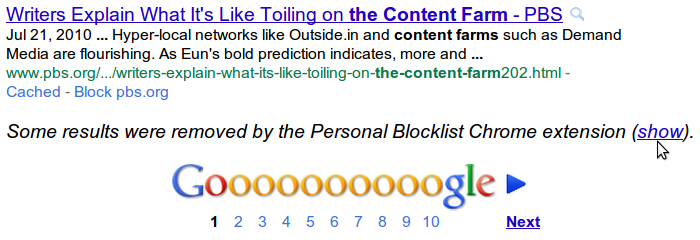
\includegraphics[width=0.8\textwidth]{rm_q.png}
  \label{fig:ejemplo}
\end{figure}
}

\frame
{
\transdissolve[duration=0.2]
\frametitle{TAKE-DOWN}
Cuando las regulaciones y leyes tiene la juridici\'on legal sobre determinados contenidos, tiene el poder para exigir y llevar a cabo la eliminaci\'on de cierto contenido o sitios web completos por ser inapropiados o ilegales.
\begin{figure}
  \centering
    
\includegraphics[width=0.5\textwidth]{ps_2.jpg}
  \label{fig:ejemplo}
\end{figure}
}

\frame
{
\transdissolve[duration=0.2]
\frametitle{INDUCED SELF-CENSORSHIP}
Esta estrategia se enfoca en limitar la exposici\'on de ciertos contenidos en Internet, fomentando la autocensura a la hora de publicar determinada informaci\'on en Internet. Esto se lleva a cabo mediante propaganda y promoci\'on de normas sociales que respeten determinados criterios sobre los contenidos aceptables, hasta la intimidaci\'on por medio de amenazas de represalias legales.
\begin{figure}
  \centering
    
\includegraphics[width=0.6\textwidth]{cens_tw.jpg}
  \label{fig:ejemplo}
\end{figure}
}


\subsection{Puntos de Control}
\frame
{
\transdissolve[duration=0.2]
\frametitle{Filtrado en la Red}
El filtrado de Internet puede ocurrir en cualquiera o cada uno de los siguientes nodos ubicados en la red.
}

\frame
{
\transdissolve[duration=0.2]
\frametitle{INTERNET BACKBONE}
Mediante determinados esquemas y tecnolog\'ias de bloqueo, se realiza un filtrado que afecta a todo el contenido que puede ser accesado por un pa\'is, esto suele ser implementado en la gateway internacional.
\begin{figure}
  \centering
    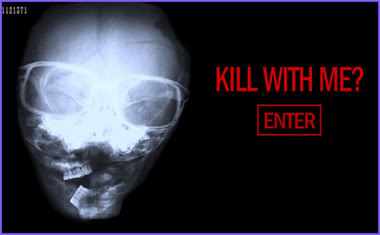
\includegraphics[width=0.5\textwidth]{cens_pop_4.jpg}
  \label{fig:ejemplo}
\end{figure}
}

\frame
{
\transdissolve[duration=0.2]
\frametitle{ISP}
Por la imposici\'on de un mandato de Gobierno o cualquier otra orden judicial, los proveedores de servicios de Internet tiene la obligaci\'on de implmentar una o cualesquiera combinaci\'on de t\'ecnicas de filtrado para bloquear el acceso a ciertos contenidos.
\begin{figure}
  \centering
    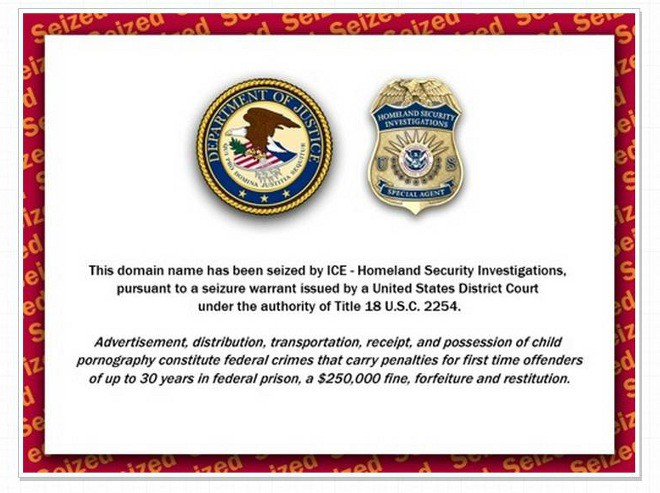
\includegraphics[width=0.6\textwidth]{bloq_int.jpg}
  \label{fig:ejemplo}
\end{figure}
}

\frame
{
\transdissolve[duration=0.2]
\frametitle{INSTITUTIONS}
Reglamentos y te\'ecnicas implementados en organizaciones, empresas, escuelas, etc., con el fin controlar y garantizar el uso adecuado de las computadoras y los accesos a Internet.
\begin{figure}
  \centering
    
\includegraphics[width=0.6\textwidth]{bloq_rs.png}
  \label{fig:ejemplo}
\end{figure}
}

\frame
{
\transdissolve[duration=0.2]
\frametitle{INDIVIDUAL COMPUTERS}
Mediante el empleo de software especializado en bloqueo y filtrado de contenidos, es posible restringir en gran medida la capacidad de las PC's individuales para acceder a determinados sitios.
\begin{figure}
  \centering
    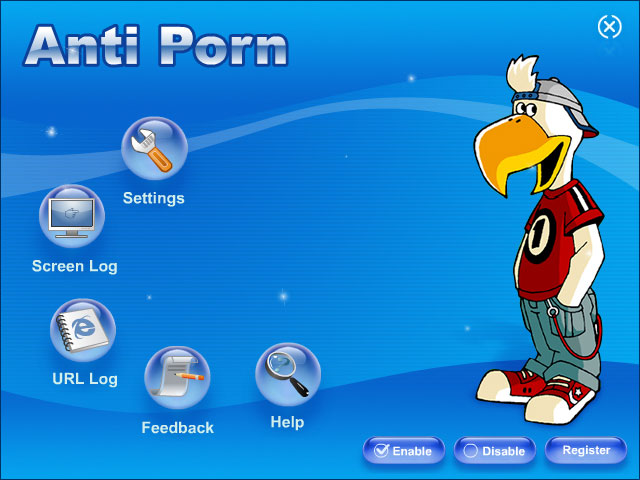
\includegraphics[width=0.5\textwidth]{bloq_ap.jpg}
  \label{fig:ejemplo}
\end{figure}
}

\frame
{
\transdissolve[duration=0.2]
\frametitle{?`C\'omo estudia el filtrado en Internet la ONI?}
\begin{itemize}
	\item Dos listas de sitios web se comprueban en cada uno de los pa\'ises analizados. Una lista global y una lista local.
	\item Mediante el uso de software de dise\~no especial, se realizan las pruebas reales a ejecutarse desde el interior de cada uno de los pa\'ises analizados.
	\item Las pruebas son variadas seg\'un: la ubicaci\'on, el ISP, la fecha, la hora, el equipo utilizado, etc. 
\end{itemize}
}



\end{document}
